%
% Interconnecting & Interfacing Quantum Networks
%

\section{Interconnecting \& interfacing quantum networks} \label{sec:inter} \index{Interfacing quantum networks}

\dropcap{A}{ny} global-scale network will inevitably comprise participants choosing to go about things their own way. The physical architecture and medium may vary from one subnetwork to the next, as may the QTCP policies they adopt. The key then is to construct efficient \textit{interconnects} between different levels of the network hierarchy, each of which may subscribe to their own QTCP policies and cross between different physical mediums. Note that the QTCP protocol presented here does not enforce any particular networking policies, but rather provides a high-level framework that can be customised essentially arbitrarily.

For example, the cost metrics and attributes employed at the intercontinental level would most certainly be very different to those in a small LAN. A small LAN might be running applications whereby they can easily reproduce packets and thereby tolerate packet loss. But for a warehouse-scale commercial quantum computing enterprise, responsible for performing one stage of a distributed quantum computation, the loss of a single packet could be extremely costly, requiring the entire computation to be performed completely from scratch due to no-cloning\index{No-cloning theorem} and no-measurement limitations, something that may not come cheaply.

Such interconnects will typically comprise a combination of:
\begin{itemize}
\item Packet switching\index{Packet!Switching}: such that packets can be arbitrarily switched between the different levels of the network hierarchy.
\item Physical interface: interconnect may be switching between different media. Such physical interfaces have costs associated with them. For example, coupling between free-space and fibre is typically very lossy. Sec.~\ref{sec:opt_inter} discusses optical interfacing with matter qubits, and Sec.~\ref{sec:hybrid} discusses hybrid architectures, where optics mediates entanglement generation between matter qubits.
\item Quantum memory\index{Quantum memory}: such that data can be buffered while it awaits its turn at being switched between networks, as different networks may have different loads and operate at different clock-rates. This is discussed in Sec.~\ref{sec:memory}.
\item Packet format conversion\index{Packet!Format conversion}: different levels of the network hierarchy may be employing entirely different cost metrics, attributes, and cost functions, requiring packet headers to be reformatted upon switching between networks.
\end{itemize}

The packet switching and quantum memory are implemented as quantum processes at nodes, using the usual quantum process formalism. The physical interface between different mediums, if there is one, could be very diverse, encompassing many types of physical systems, but can always be characterised using the quantum process formalism. Packet headers, which contain all formatting, cost, and routing information are represented entirely classically and communicated entirely by the classical network. Thus, this operation also takes place at nodes, but no quantum processes are taking place.

%
% Optical Interfacing
%

\subsection{Optical interfacing} \label{sec:opt_inter} \index{Optical!Interfacing}

Unless the entire pipeline of quantum operations through the course of a protocol is all-optical, there will be a need to exchange information between physical systems, for example via light-matter interactions \cite{bib:Cohen-Tannoudji92}. We will now discuss optical interfacing with some of the significant types of matter systems, such that their intercommunication can be optically mediated over the network.

%
% Two-Level Systems
%

\subsubsection{Two-level systems} \index{2-level systems}

The archetypal interface is that between a photonic qubit in the \mbox{$\{\ket{0},\ket{1}\}$} photon-number basis, and a two-level matter qubit\index{Matter qubits} in the $\ket{g}$ (ground) and $\ket{e}$ (excited) state basis. The logical qubit is defined as,
\begin{align}
	\ket{0}_L &\equiv \ket{g}, \nonumber \\
	\ket{1}_L &\equiv \ket{e}.
\end{align}.
Examples include atoms in cavities\index{Atoms in cavities}, NV centres\index{Nitrogen-vacancy (NV) centres}, and engineered quantum dots\index{Quantum dots}.

In the case of a photon interacting with a two-level matter qubit, the interface can be expressed via the Jaynes-Cummings\index{Jaynes-Cummings Hamiltonian} interaction Hamiltonian of the form,
\begin{align} \label{eq:two_level_hamil}
\hat{H}_\mathrm{int} = \hbar \chi (\hat{a}\,\hat\sigma^+ + \hat{a}^\dag\hat\sigma^-),
\end{align}
where $\hat{a}$ ($\hat{a}^\dag$) is the photonic annihilation (creation) operator, $\hat\sigma^\pm$ are the Pauli spin-flip operators, and $\chi$ is the interaction strength\index{Interaction strength}. The interpretation of this Hamiltonian is very clear upon inspection -- the annihilation (creation) of a photon is associated with the excitation (relaxation) of the two-level matter system, thereby directly coherently exchanging quantum information between the two systems, as shown in Fig.~\ref{fig:opt_int}.

\begin{figure}[!htbp]
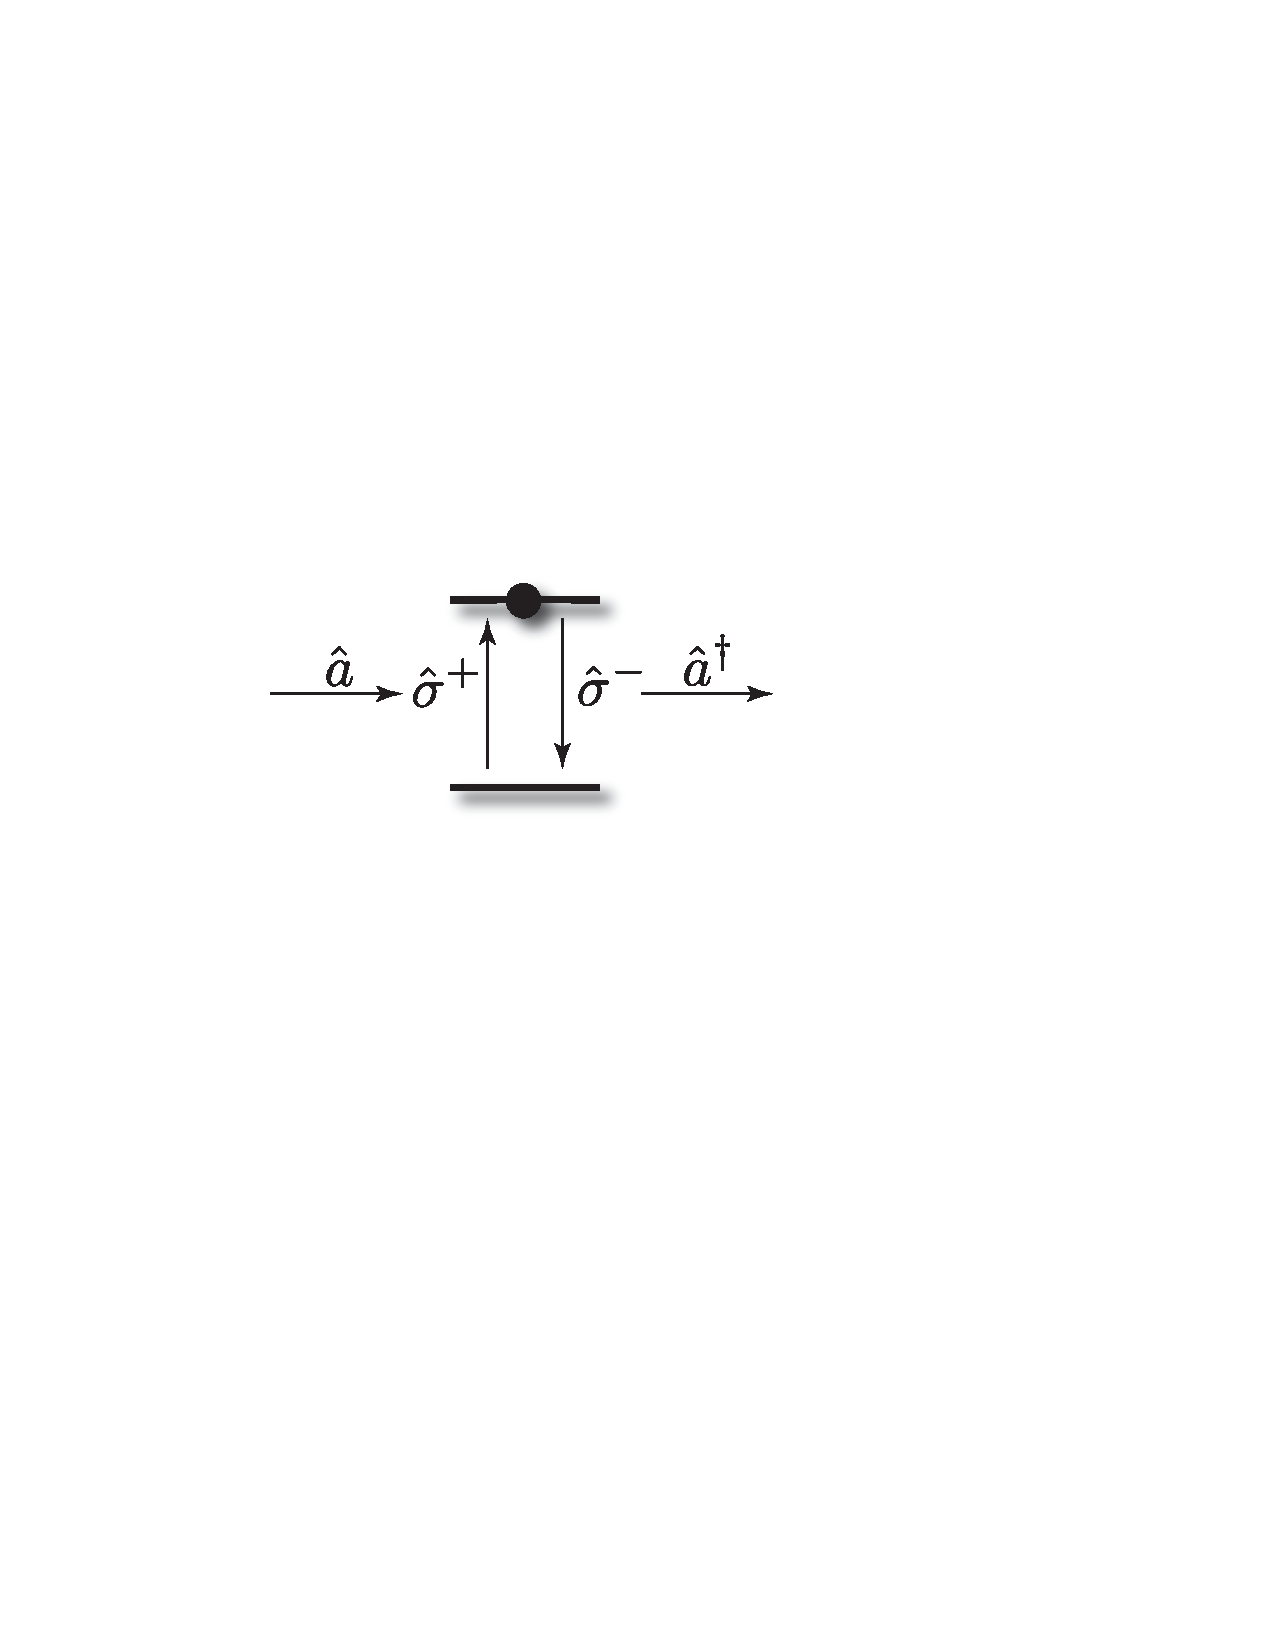
\includegraphics[clip=true, width=0.3\textwidth]{opt_inter}
\captionspacefig \caption{Light-matter interfacing between a single-photon state ($\hat{a}$, $\hat{a}^\dag$) and a two-level matter qubit ($\ket{g}$, $\ket{e}$). The absorption (emission) of a photon is associated with the excitation (relaxation) of the matter qubit ($\hat\sigma^\pm$).} \label{fig:opt_int}
\end{figure}

%
% Lambda-Configuration Systems
%

\subsubsection{$\lambda$-configuration systems} \index{$\lambda$-configuration systems}

Alternately, one can easily optically interface with a $\lambda$-configuration system, as shown in Fig.~\ref{fig:lambda_atom}. Here there are two degenerate ground states representing the logical qubit basis states (\mbox{$\ket{0}_L\equiv\ket{\!\uparrow}$}, \mbox{$\ket{1}_L\equiv\ket{\!\downarrow}$}), one of which may undergo a transition to an excited state, $\ket{e}$. By pumping the system to the excited state and waiting for a coherent relaxation, the emitted photon may be used to couple the qubit state of the $\lambda$-configuration to an optical mode, mapping the qubit value of the matter qubit to a photon-number representation.

\begin{figure}[!htbp]
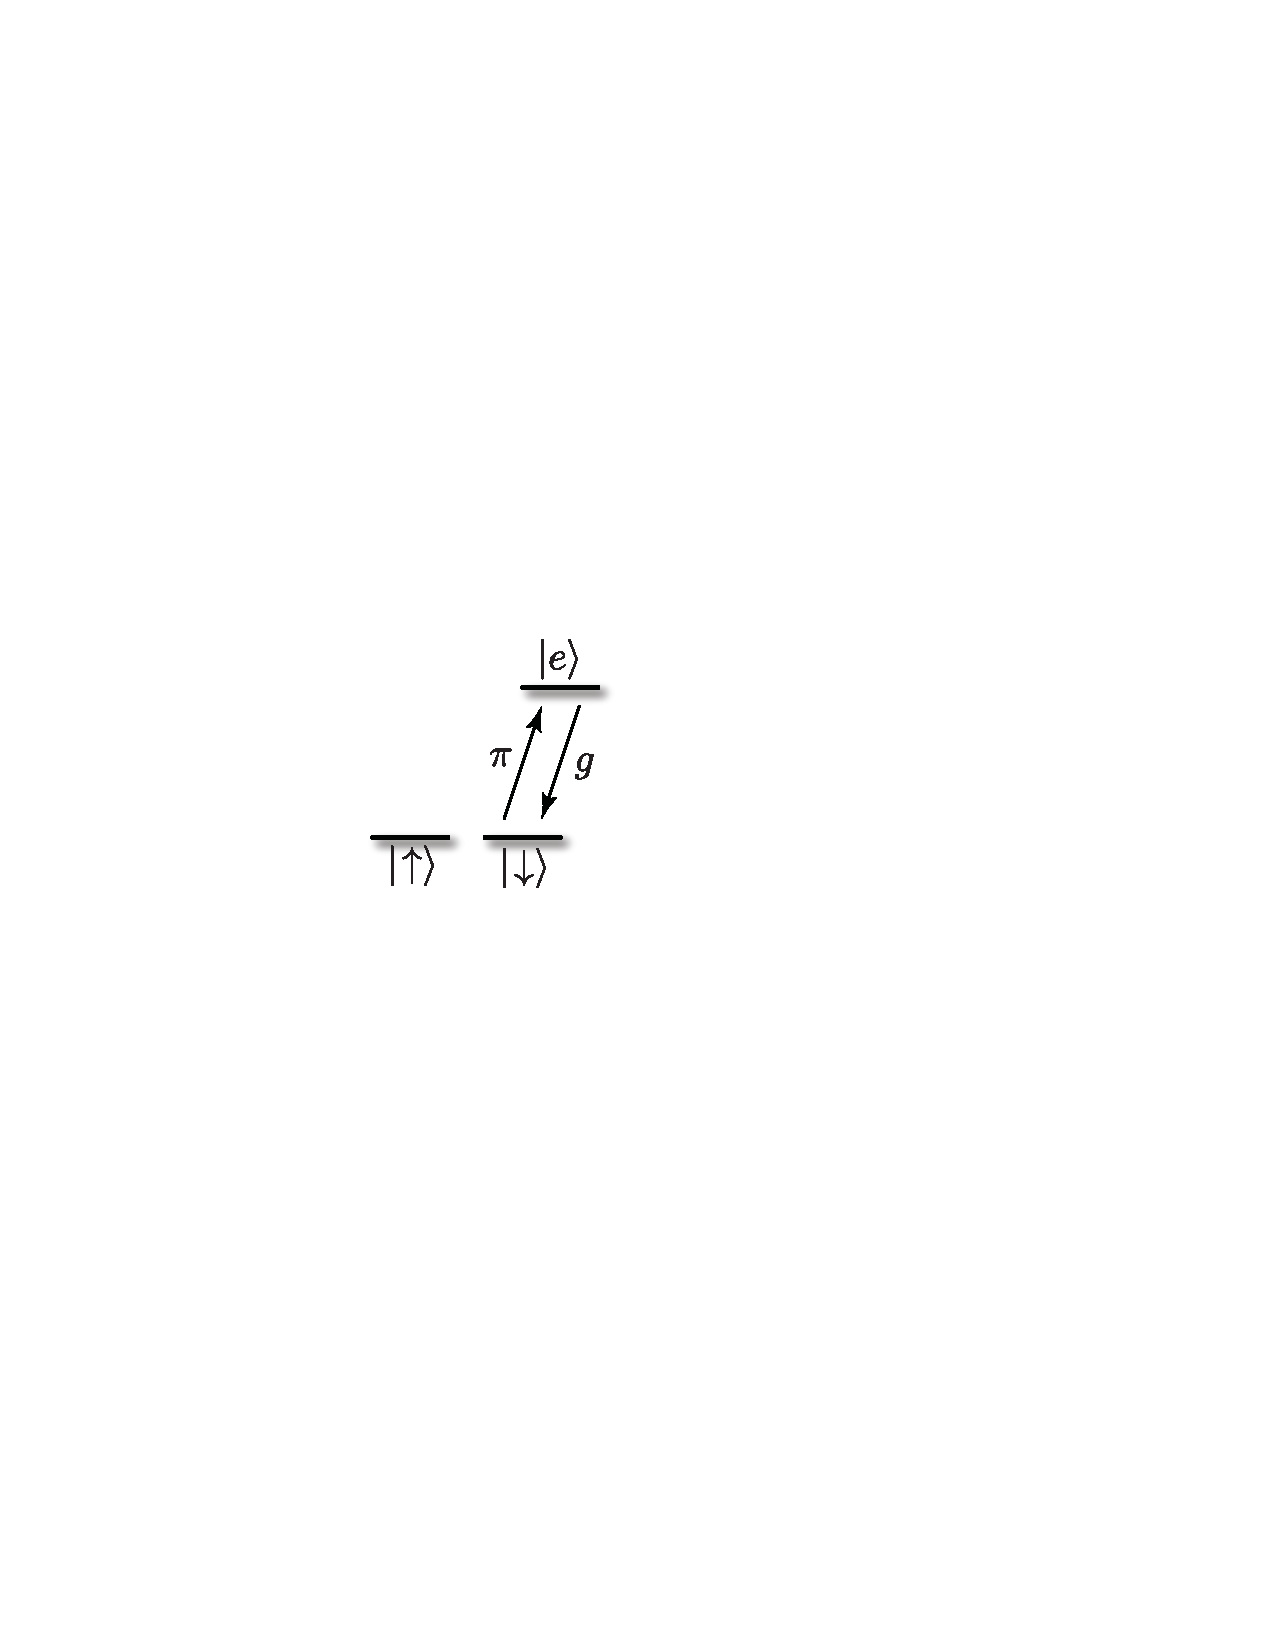
\includegraphics[clip=true, width=0.225\textwidth]{lambda_atom}
\captionspacefig \caption{Light-matter interfacing between an optical mode and a $\lambda$-configuration system. The two degenerate ground states represent the logical qubit (\mbox{$\ket{0}_L\equiv\ket{\!\uparrow}$}, \mbox{$\ket{1}_L\equiv\ket{\!\downarrow}$}), only one of which may undergo transition to the excited state $\ket{e}$. Upon pumping the \mbox{$\ket{\!\downarrow}\to\ket{e}$} transition with a $\pi$-pulse, a relaxation back to the ground state maps the logical qubit value to photon-number.} \label{fig:lambda_atom}
\end{figure}

%
% Atomic Ensembles
%

\subsubsection{Atomic ensembles} \label{sec:atomic_ens} \index{Atomic ensembles}

In addition to single atoms with well-defined electronic structure, atomic ensembles \cite{DLCZ, bib:Chou05} can be used, whereby the absorption of a photon creates a \textit{collective excitation}\index{Collective excitations} -- a superposition of a single excitation across all the atoms in the ensemble. Specifically, excitations are represented using collective excitation operators,
\begin{align}\index{Collective excitations!Operator}
\hat{S}^\dag = \frac{1}{\sqrt{N}}\sum_{i=1}^N \hat{S}_i^\dag,
\end{align}
where,
\begin{align}
\hat{S}_i^\dag=\ket{e}_i\bra{g}_i,
\end{align}
is the excitation operator for the $i$th atom in the ensemble, $\ket{g}_i$ and $\ket{e}_i$ are the ground and excited states for the $i$th particle, and there are $N$ atoms. The state of a single collective excitation is then given by,
\begin{align}
\ket{\psi_\mathrm{collective}} = \hat{S}^\dag \ket{g}^{\otimes N}.	
\end{align}

Atomic ensembles are essentially well-engineered clouds of atomic gasses, trapped in a glass container, coupled to an optical mode. Atomic ensembles have been demonstrated with extremely long coherence lifetimes ($T_2$-times on the order of milliseconds\index{T$_2$-time}), operating at room temperatures (a very attractive feature on its own). They exhibit \textit{collective enhancement}\index{Collective enhancement} in their coupling to the optical mode -- the optical coupling strength is amplified by a factor quadratic in $N$ compared to single-atom optical coupling, mitigating the need for a cavity.

The collective excitations exhibit the same general mathematical structure as single-atom excitations -- the absorption (emission) of a single photon is associated with a single collective excitation (relaxation), albeit with the favourable collective enhancement in the coupling strength.

To couple with a polarisation-encoded photonic qubit, a PBS can be employed to spatially separate the horizontal and vertical modes, each of which couples to a separate atomic ensemble, which jointly represent the logical qubit, as shown in Fig.~\ref{fig:atomic_ensemble_qubit}.

\begin{figure}[!htbp]
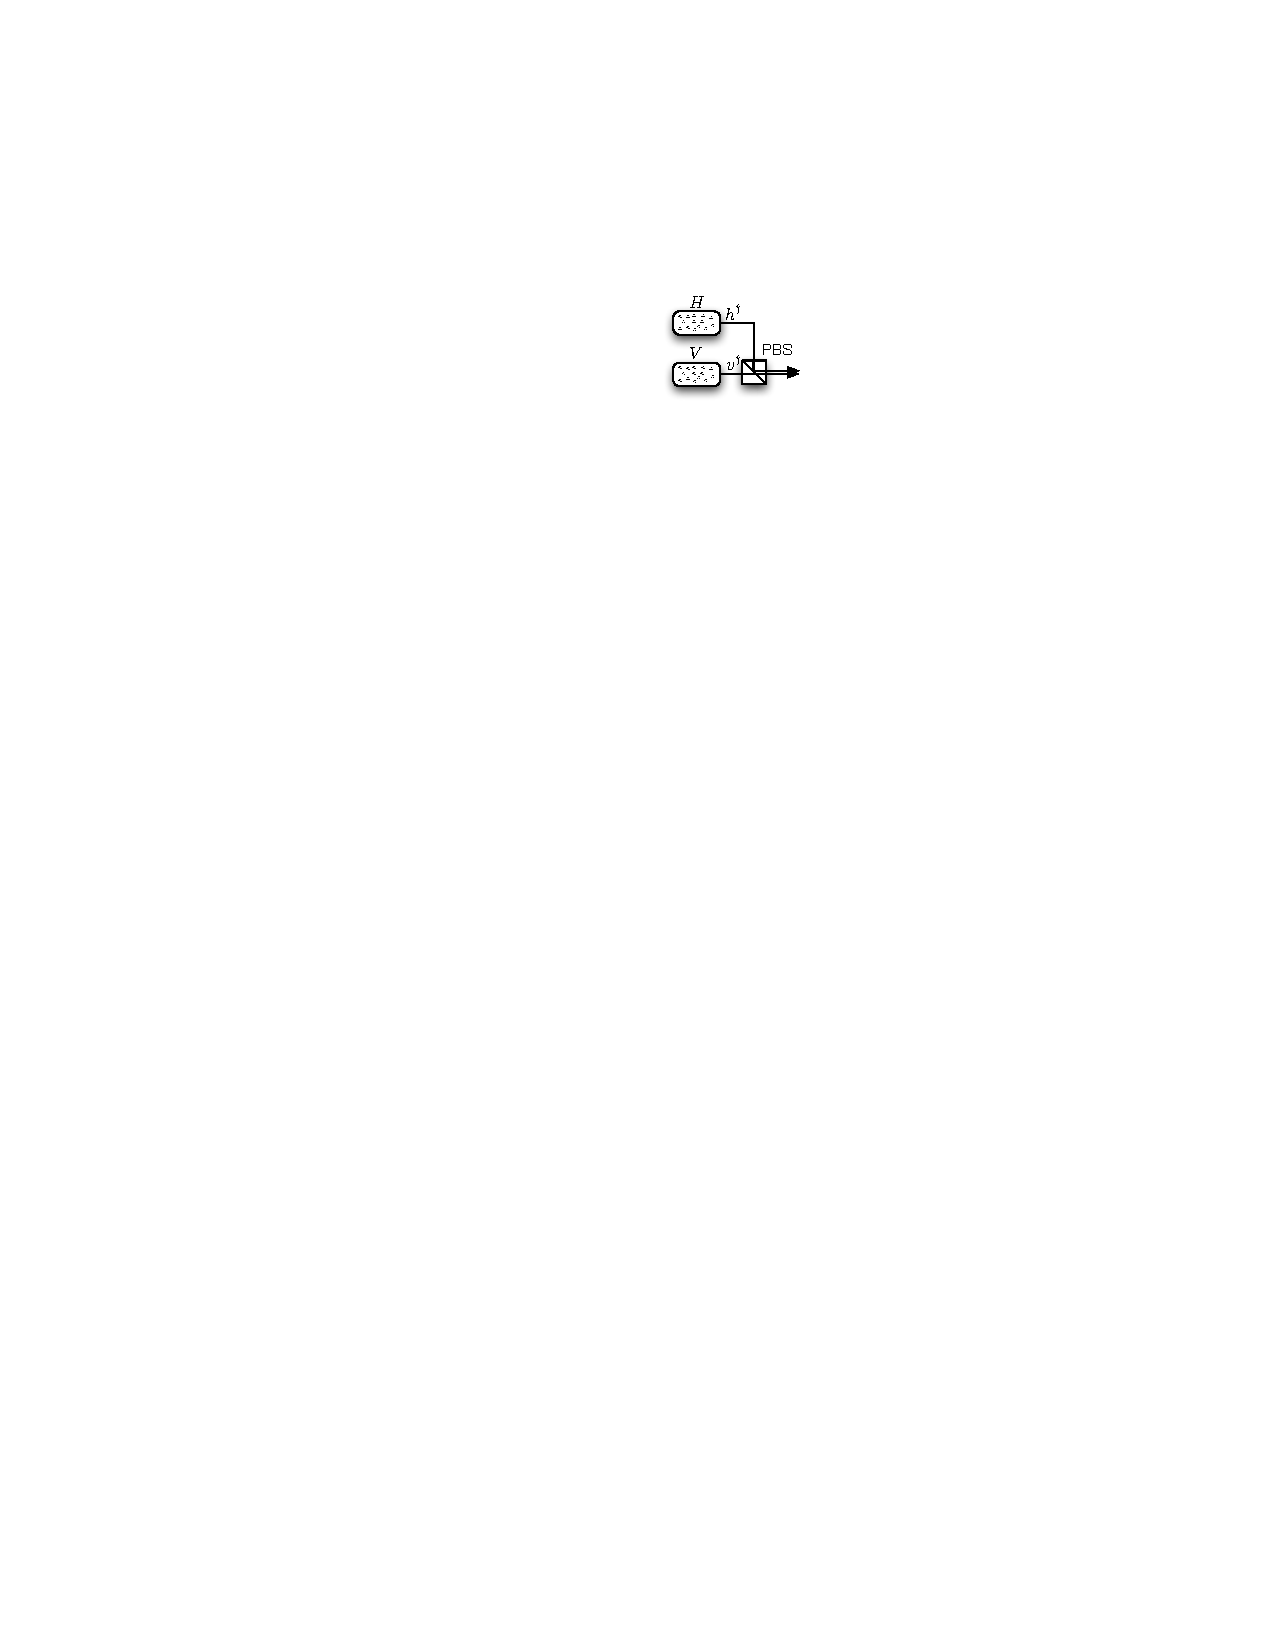
\includegraphics[clip=true, width=0.225\textwidth]{atomic_ensemble_qubit}
\captionspacefig \caption{Coupling a polarisation-encoded photonic qubit to a pair of atomic ensembles, each of which corresponds to one of the qubit's logical basis states ($\ket{0}$ or $\ket{1}$). The horizontal and vertical components of the photonic qubit are spatially separated using a PBS, which subsequently independently interface with distinct atomic ensembles via collective excitation.} \label{fig:atomic_ensemble_qubit}
\end{figure}

Atomic ensembles have been proposed as quantum memories, given their long coherence lifetimes. Additionally, a protocol for universal cluster state quantum computation (Sec.~\ref{sec:CSQC}) based upon atomic ensemble qubits has been described \cite{bib:RohdeAtEns10}.

Essentially, the long coherence lifetimes of collective excitations owes to the fact that the excitation is effectively encoded as a W-state (Sec.~\ref{sec:W_state_prep})\index{W-states}, an equal superposition of a single excitation across many ($N$) atoms, of the form,
\begin{align}
\ket{\psi_W^{(N)}} = \frac{1}{\sqrt{N}}(&\ket{e,g,g,\dots}\nonumber \\
+&\ket{g,e,g,\dots}\nonumber \\
+&\ket{g,g,e,\dots}\nonumber \\
+&\dots\nonumber \\
+&\ket{g,g,\dots,e}).
\end{align}
W-states are favourable from a decoherence perspective as tracing out a single particle has minimal impact on the coherence of the residual state, which preserves most entanglement, with this robustness growing with the number of particles. This is in stark contrast to GHZ states, which completely decohere under the loss of just a single particle.

Specifically, if $\ket{\psi_W^{(N)}}$ is the $N$-particle W-state (collective excitation), tracing out a single particle yields,
\begin{align}
\hat\rho_\mathrm{tr} &= \mathrm{tr}_1(\ket{\psi_W^{(N)}}\bra{\psi_W^{(N)}}) \\
&= \left(1-\frac{1}{N}\right)\ket{\psi_W^{(N-1)}}\bra{\psi_W^{(N-1)}} + \frac{1}{N}(\ket{g}\bra{g})^{\otimes (N-1)}, \nonumber
\end{align}
which for \mbox{$N\gg 1$} approaches the pure state $\ket{\psi_W^{(N-1)}}$, i.e a W-state with one fewer particles.

%
% Superconducting Qubits
%

\subsubsection{Superconducting qubits}\label{sec:superconducting_qubits}\index{Superconducting qubits}\index{Quantum transducers}\index{Microwave qubits}

In the context of superconducting qubits (Sec.~\ref{sec:artificial_atoms}), the energy difference between the energy levels being utilised to encode the qubit is extremely small. Therefore photons coupled to these transitions sit in the microwave regime, whose wavelength lies in the range \mbox{$\lambda\sim100\mu$m-1m}.

%To build a scalable quantum computer, multiple qubits are required, with the ability to interact with one another. Hence, it is essential to find ways to transfer quantum information between distinct superconducting qubits. When doing so, it is essential that quantum coherence be preserved. This implies we need to find a different kind of qubit, which can carry information from one place to another, but interacts only weakly with the other qubits and the environment. Photons are the ideal candidate for this (Sec.~\ref{sec:opt_enc_of_qi}). Photonic qubits for carrying information should have frequencies equal to the energy difference between qubit levels. For a superconducting qubit, the energy difference is very small, hence the frequency of optical qubits is in microwave regime, .

Information transfer between distinct superconducting qubits is achieved using a resonator, which acts as a quantum data bus\index{Quantum data bus}. A simple resonator\index{Resonators} is an LC circuit\index{LC circuit}, which can support only one frequency mode, but a waveguide resonator can support multiple modes. In general, the transmission line circuits used in non-linear quantum electric circuits\index{Non-linear quantum electric circuits} are in the form of coplanar waveguides\index{Waveguides}. These waveguides are engineered to handle a particular set of frequencies, and produce transmission lines with tuneable frequency. Tuneable resonators\index{Tuneable resonators} are very important in quantum optics, and are useful in implementing controllable coupling between different quantum elements, and also in shaping photon wave-packets. 

In cavity quantum electrodynamics (QED)\index{Quantum electrodynamics} the interaction of a natural atom with an optical photon in the visible wavelength regime is considered. Similarly, the interaction between quantum non-linear electrical circuits and  microwave photons are investigated in circuit QED. The coupling-strength between a natural atom and visible light photon is fixed, where atoms couple weakly with photons \cite{bib:raimond2001manipulating}. Meanwhile, the coupling-strength between a superconducting qubit and a microwave can be manipulated by engineering the parameters of the qubit and resonator, yielding strong and ultra-strong coupling\index{Strong coupling}\index{Ultra-strong coupling} between qubits and photons \cite{bib:wallraff2004strong} (see Fig.~\ref{fig:microwave_qubits}). Furthermore, the coupling between an atom and a photon can be tuned dynamically during the course of an experiment. Several quantum optics components such as mirrors, beamsplitters, circulators and switches can also be designed based on quantum electric circuits.

\begin{figure}[!htbp]
\if 2\pubmode
	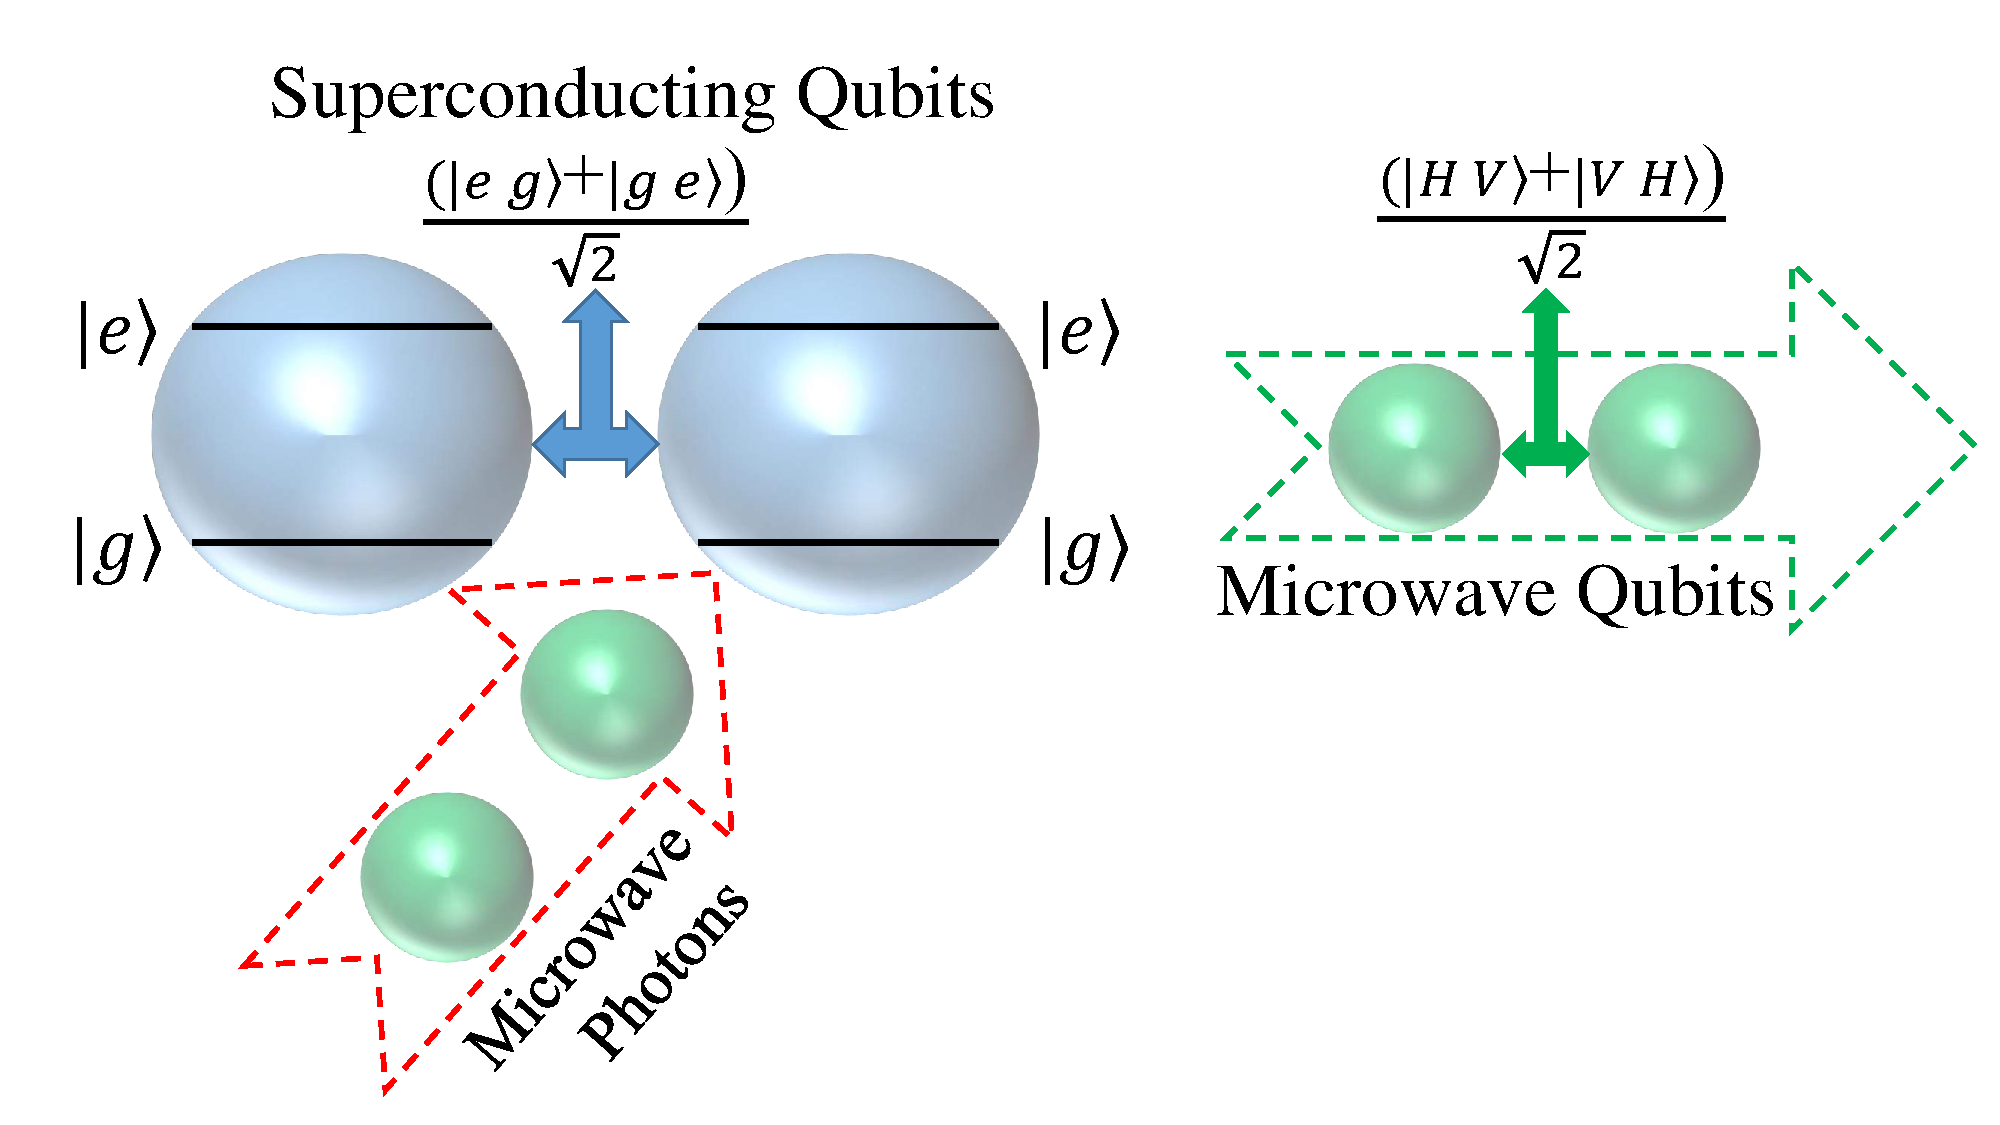
\includegraphics[clip=true, width=0.475\textwidth]{microwave_qubits}
\else
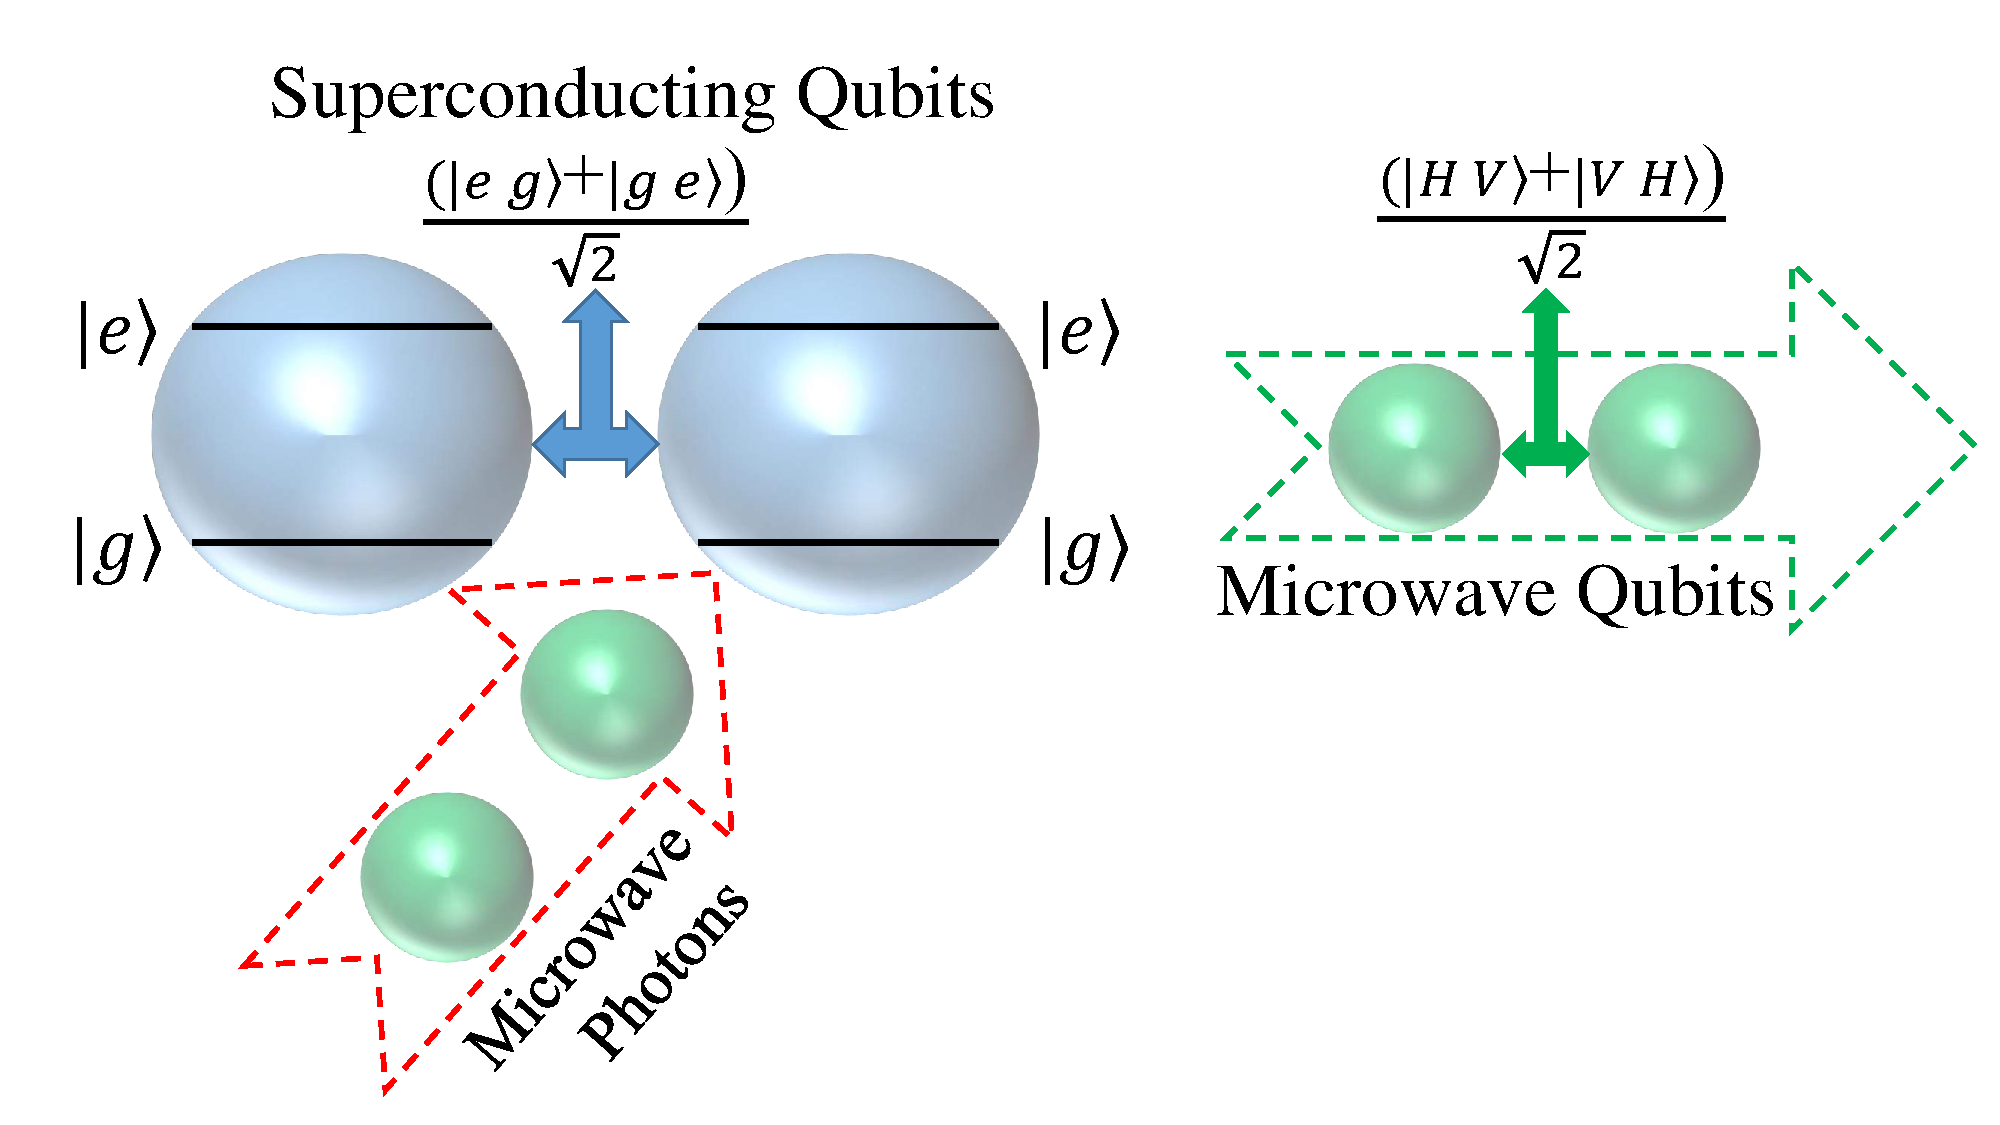
\includegraphics[clip=true, width=0.7\textwidth]{microwave_qubits}
\fi
\captionspacefig \caption{Schematic sketch of the interaction between superconducting qubits and microwave qubits. The superconducting qubits are in the entangled state \mbox{$\frac{1}{\sqrt{2}}(\ket{e,g} + \ket{g,e})$}, where $\ket{g}$ and $\ket{e}$ are the ground and excited states of the superconducting qubits. These are subjected to interact with the flying qubits, the microwave qubit (red dashed arrow). The photons become entangled and the output state of the photons are \mbox{$\frac{1}{\sqrt{2}}(\ket{H,V} + \ket{V,H})$}, where $\ket{H}$ and $\ket{V}$ are the horizontal and vertical polarisation modes respectively.}\label{fig:microwave_qubits}\index{Microwave qubits}
\end{figure}

%\subsubsection{Quantum transducers}

Due to scalability requirements, superconducting qubits are the most widely used qubit implementation used today. The energy-level spacing in superconducting qubits lie in the microwave regime. Hence to control and transfer information from a superconducting qubit one might need to use microwave photons. In principle, we can use microwave photons to transfer information from one node to another, but such a transmission process is extremely lossy. Also, such processes have very demanding technical requirements, like the design of specialised Niobium waveguides\index{Niobium waveguides}, maintained at extremely low temperatures. Hence it isn't feasible to use microwave photons for the long-distance transfer of quantum information. Meanwhile, it is well known that photons in the visible spectrum can be transmitted easily using optical fibres, with favourable efficiency.

To convert microwave photons to optical photons we can use a quantum transducer. A sketch of a typical design for a quantum transducer\index{Quantum transducers} is shown in Fig.~\ref{fig:quantum_transducer} through a flowchart diagram. The quantum computer is made up of superconducting qubits, which feed quantum information to microwave qubits. The microwave qubits are then interfaced to optical qubits in the visible spectrum through a 3-level quantum system\index{3-level systems}, which can couple at both microwave and optical frequencies. These steps should be reversible. Hence it should be possible to convert the optical qubits back into microwave qubits at the receiving end. 

\begin{figure}[!htbp]
\if 3\pubmode
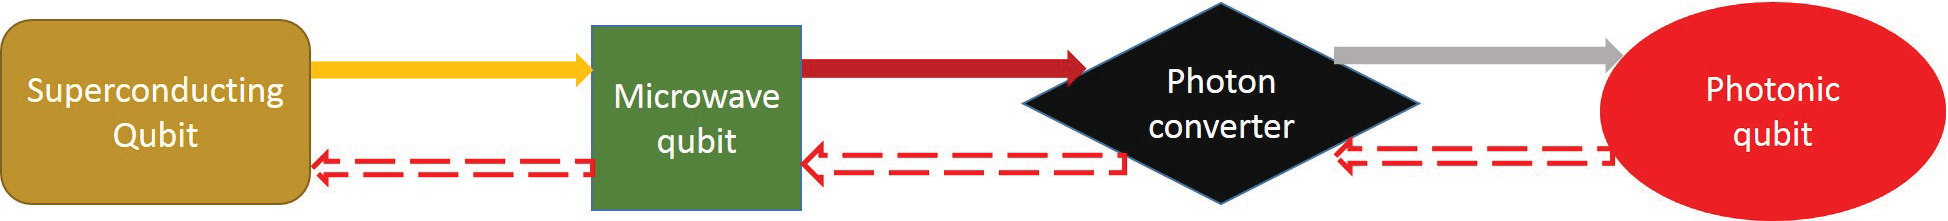
\includegraphics[clip=true, width=\textwidth]{quantum_transducer}
\else
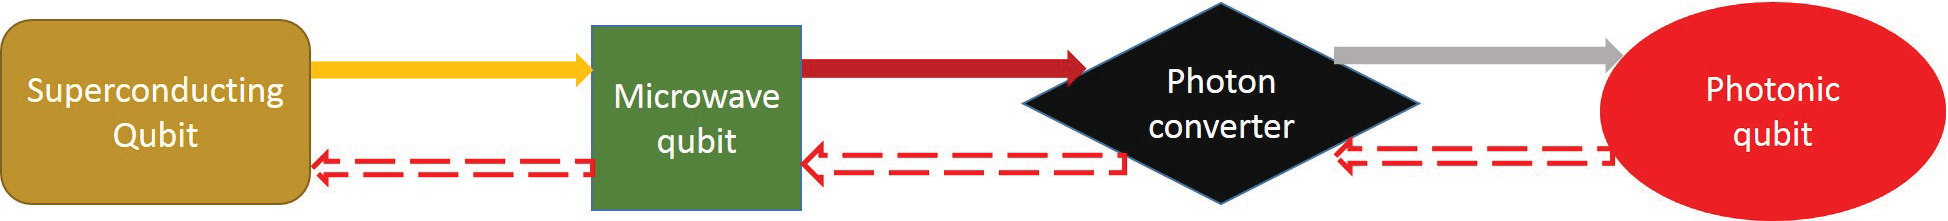
\includegraphics[clip=true, width=0.475\textwidth]{quantum_transducer}
\fi
\captionspacefig \caption{Block diagram for the quantum transducer. The quantum computer comprising superconducting qubits couples with the microwave qubit. The microwave qubit and the photonic qubit are coupled by a three-level system in which the energy difference between the levels correspond to both microwave and visible optical frequencies. The thick arrows denote the forward process, required to convert the microwave to optical frequencies, and the dashed arrows represent the reverse process, required at the receiving end to convert the optical frequency to a microwave frequency.}\label{fig:quantum_transducer}
\end{figure}

There are several proposals for quantum transducers in existence and they can be classified into two major classes:
\begin{itemize}
	\item Opto-mechanical \cite{bib:rabl2010quantum, bib:barzanjeh2011entangling, bib:bochmann2013nanomechanical, bib:didier2014quantum, bib:schuetz2015universal, bib:shumeiko2016quantum, bib:stannigel2010optomechanical}.
	\item Spin-ensembles \cite{bib:imamouglu2009cavity, bib:blum2015interfacing}.
\end{itemize}

The opto-mechanical quantum transducer\index{Opto-mechanical quantum transducer} (see Fig.~\ref{fig:opto_mechanics_transducer}), as the name suggests, combines optical components with a nano-mechanical resonator and converts the microwave photon\index{Phonons} into a phonon (acoustic) mode. The acoustic mode is then transmitted via waveguides\index{Waveguides}. Since we need to fabricate waveguides with very high precision to transmit phonon modes, this scheme is not suitable for communicating between two distant quantum computers. A coupling of the phonon mode to the optical photon mode in the visible region was suggested to enable long-distance transfer of quantum information.

\begin{figure}[!htbp]
\if 3\pubmode
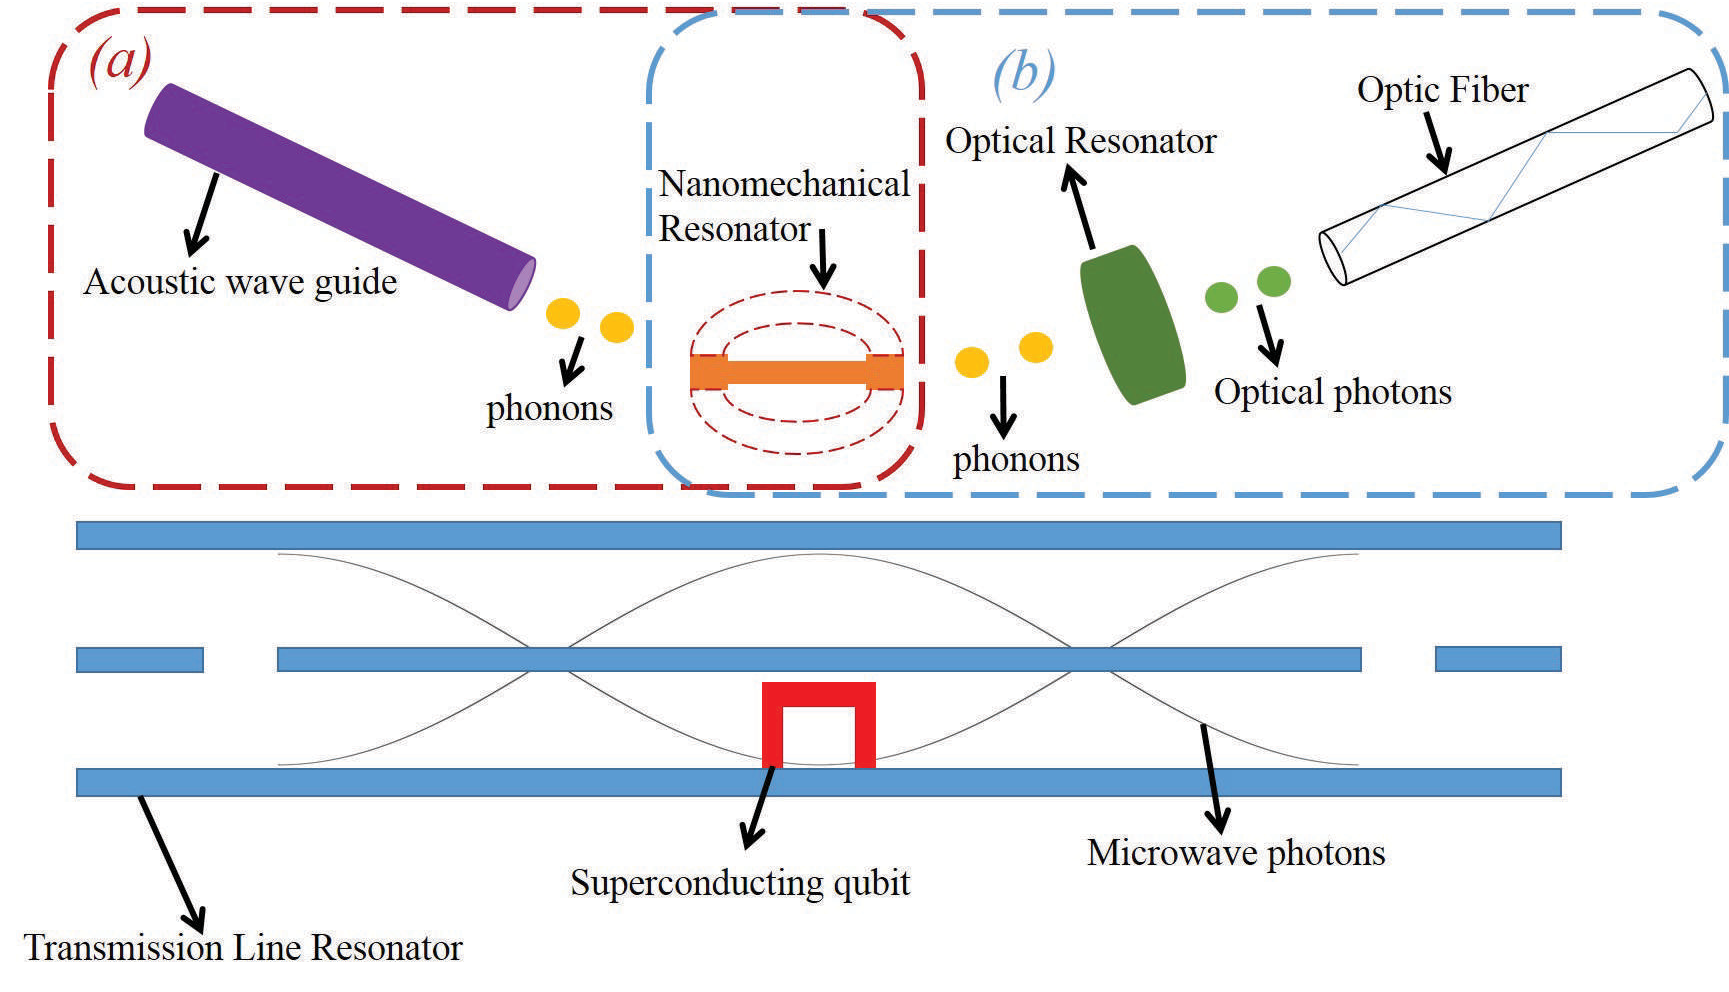
\includegraphics[clip=true, width=\textwidth]{transducer_scheme_1}
\else
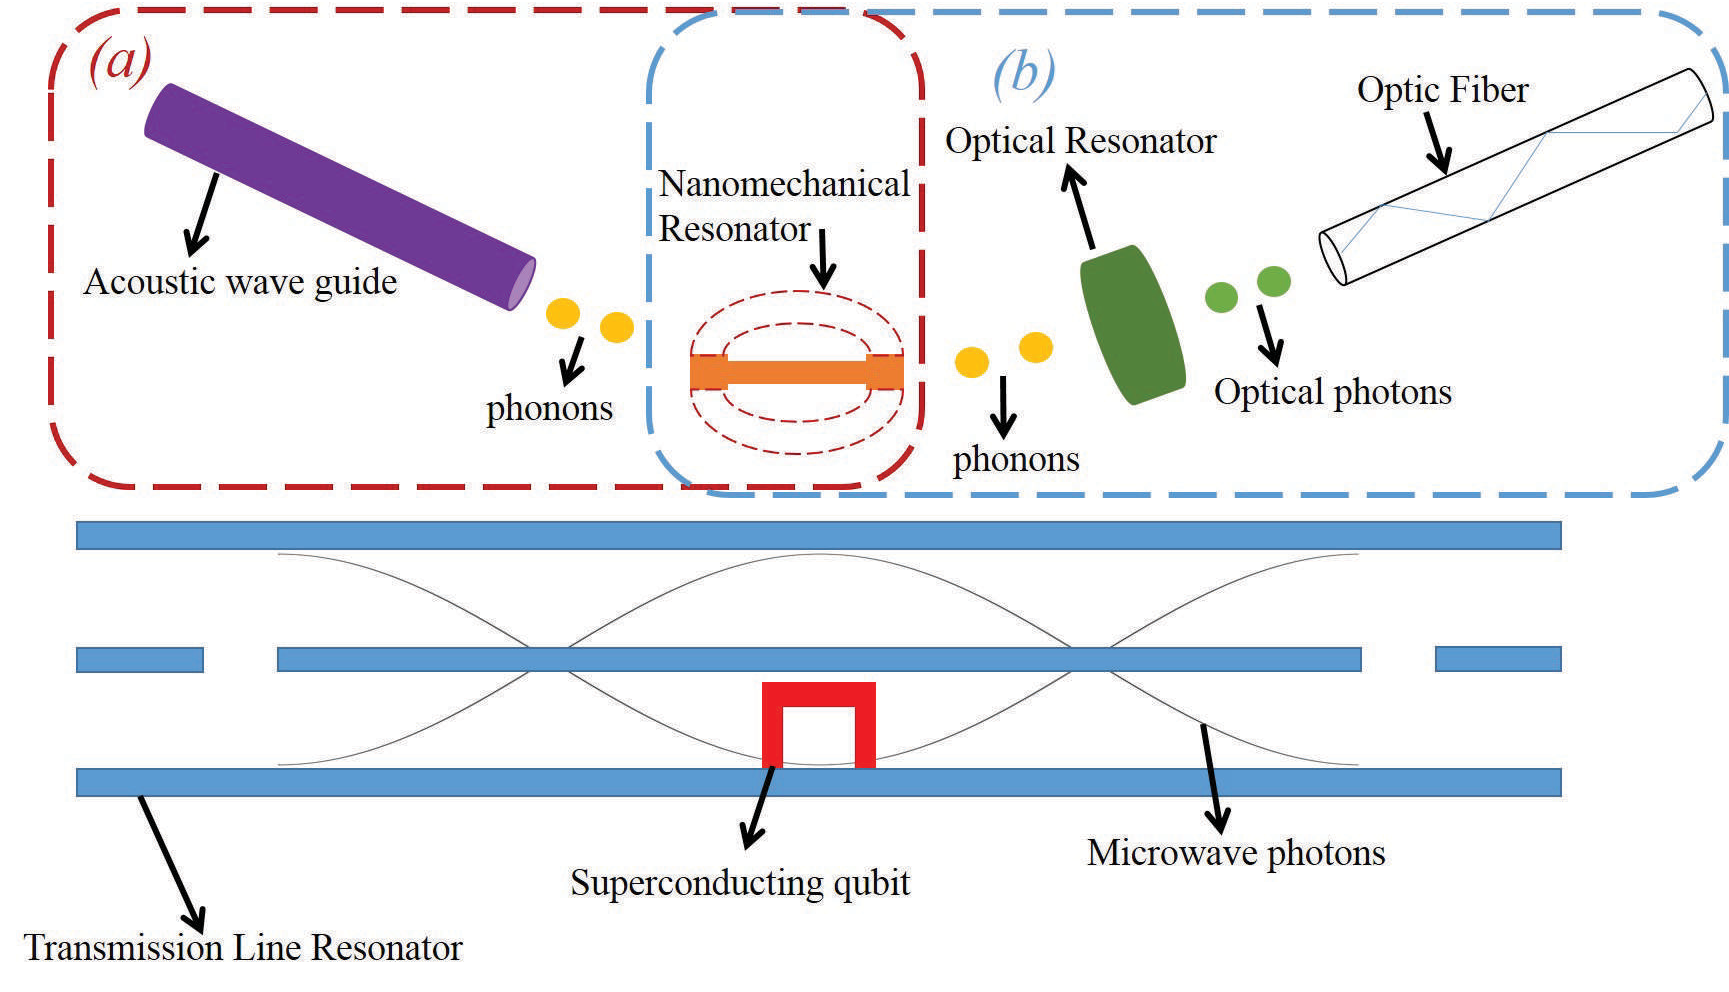
\includegraphics[clip=true, width=0.475\textwidth]{transducer_scheme_1}
\fi
\captionspacefig \caption{Scheme for an opto-mechanics-based quantum transducer. There are two possible ways of converting microwaves. The final steps for the process in which acoustic modes are transported using waveguides is enclosed by a brown coloured box with dashed outlines labeled (a). Similarly the blue coloured box labeled (b) represents the scheme where phonons are converted to optical photons which are then transmitted via optical fibres. The initial few steps consisting of the superconducting qubit, transmission line resonator and microwaves are common to both processes.}\label{fig:opto_mechanics_transducer}\index{Opto-mechanical quantum transducer}
\end{figure}

The Hamiltonian of an opto-mechanical quantum transducer, which converts a microwave photon to optical photon using an intermediate nano-mechanical resonator\index{Nano-mechanical resonator} reads,
\begin{align}
\hat{H} &= \hbar \omega_{1} \, \hat{a}_{1}^{\dag} \hat{a}_{1} + \hbar \omega_{2} \, \hat{a}_{2}^{\dag} \hat{a}_{2} \nonumber\\
&+ \hbar \Omega \, \hat{b}^{\dag} \hat{b} + \hbar \, g \, (\hat{b}+\hat{b}^{\dag}) (\hat{a}_{2}^{\dag} \hat{a}_{1} + \hat{a}_{1}^{\dag} \hat{a}_{2}),
\end{align}
where $\omega_{1}$ ($\omega_{2}$) is the frequency of the microwave (optical) photon, and $\Omega$ is phonon frequency. The operators $\hat{a}_{1}$ ($\hat{a}_{1}^{\dag}$) and $\hat{a}_{2}$ ($\hat{a}_{2}^{\dag}$) denote the annihilation (creation) operators corresponding to the microwave and optical photons respectively. Meanwhile, $\hat{b}^{\dag}$ ($\hat{b}$) denotes the phonon creation (annihilation) operator corresponding to the phonons. The factor $g$ is the coupling-strength between the microwave, phonon and photon modes. This design for a quantum transducer is widely preferred, since the optical photons in the visible spectrum can be transmitted over long distances using fibre optics. But the scheme requires two intermediate conversions, each of which reduces overall efficiency.

The spin-ensemble-based quantum transducer\index{Spin-ensemble quantum transducer} (see Fig.~\ref{fig:spin_ens_transducer}) is an alternative to the opto-mechanical quantum transducer. In this scheme an ensemble of spins interact with microwave qubits via magnetic dipole coupling\index{Magnetic dipole coupling}, while the superconducting qubits interact via electric dipole coupling\index{Electric dipole coupling} with the microwave coupling. The Hamiltonian for such a system is,
\begin{align}
\hat{H} = \hat{H}_{\mathrm{mw}} + \hat{H}_{\mathrm{spin}} + \hat{H}_{\mathrm{opt}},
\end{align}
where,
\begin{align}
\hat{H}_{\mathrm{mw}} &= \hbar \omega_\mathrm{sq} \hat\sigma_\mathrm{sq}^{\dag} \hat\sigma_\mathrm{sq} + \hbar \omega_{\mu} \hat{a}^{\dag} \hat{a} + \hbar g_{\mu} (\hat{a}^{\dag} \hat\sigma_\mathrm{sq} + \hat{a} \hat\sigma_\mathrm{sq}^{\dag}),\nonumber \\
\hat{H}_{\mathrm{spin}} &= \hbar g_\mathrm{s} (\hat\sigma_\mathrm{ba}^{\dag} \hat\sigma_\mathrm{ba} + \hat\sigma_\mathrm{bs}^{\dag} \hat\sigma_\mathrm{bs}), \nonumber\\
\hat{H}_{\mathrm{opt}} &= \hbar g_\mathrm{ab} (\hat\sigma_\mathrm{ba}^{\dag} \hat{c} + \hat{c}^{\dag} \hat\sigma_\mathrm{ba}).
\end{align}

\begin{figure}[!htbp]
\if 3\pubmode
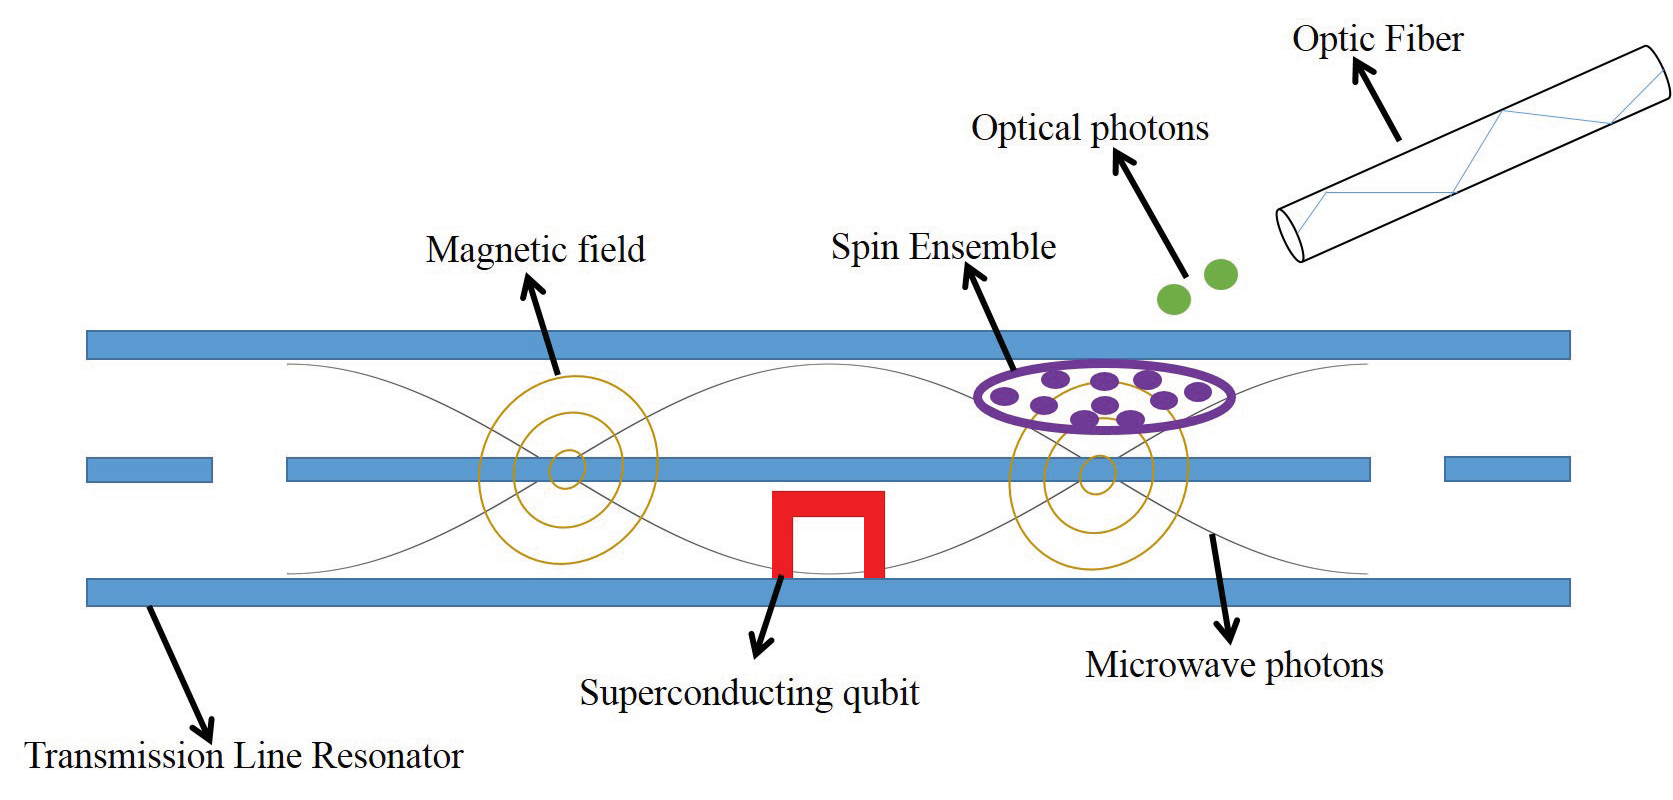
\includegraphics[clip=true, width=0.9\textwidth]{transducer_scheme_2}
\else
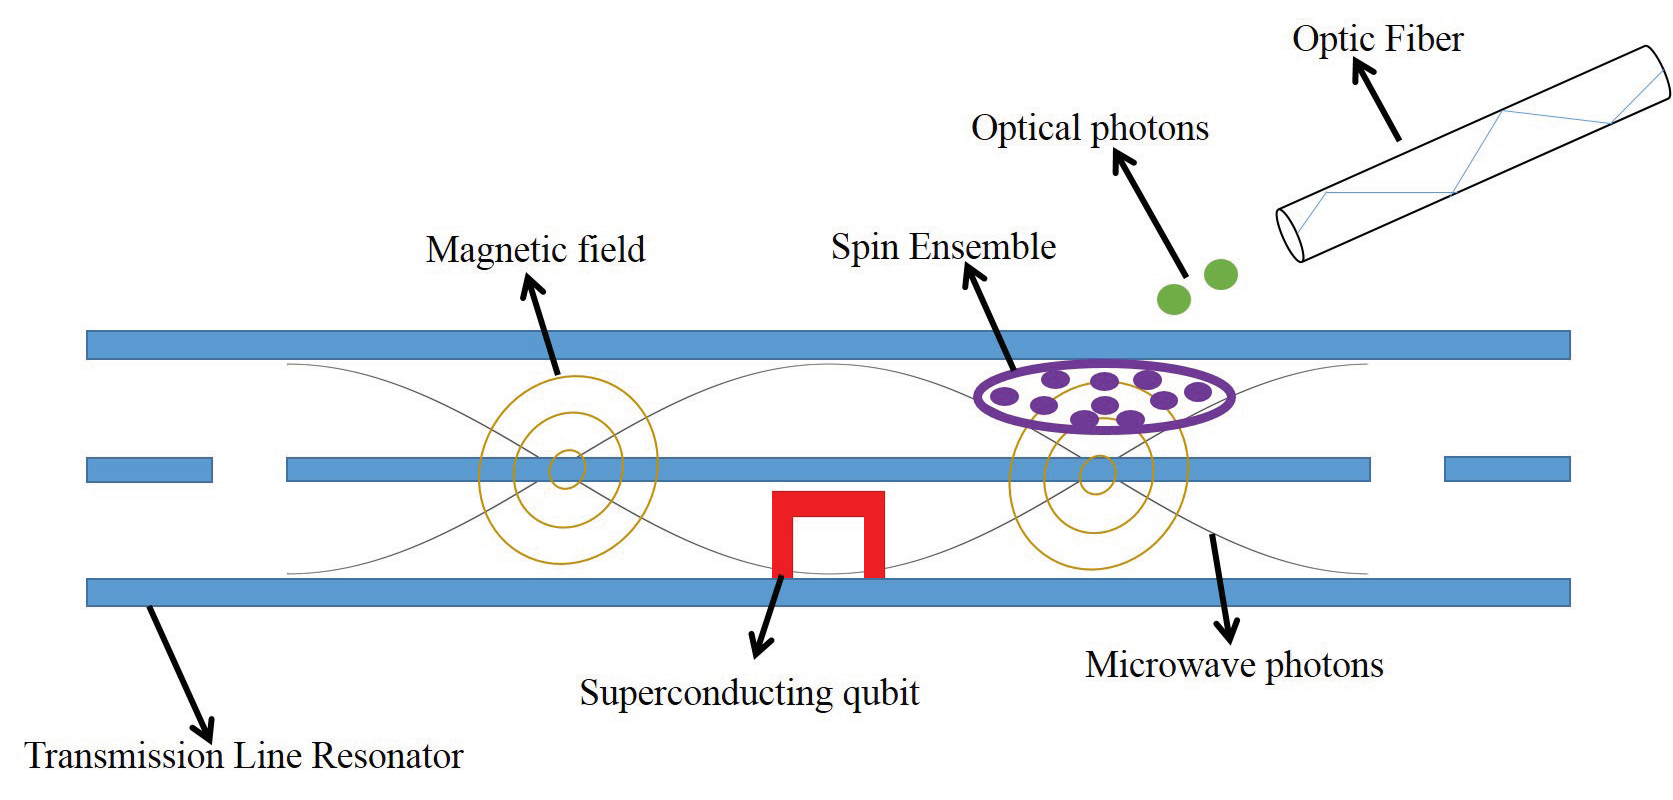
\includegraphics[clip=true, width=0.475\textwidth]{transducer_scheme_2}
\fi
\captionspacefig \caption{The spin-ensemble-based quantum transducer. Microwave photons are converted to optical photons via a spin-ensemble.}\label{fig:spin_ens_transducer}\index{Spin-ensemble quantum transducer}
\end{figure}

The factor $\omega_\mathrm{sq}$ is the frequency of the superconducting qubit, and $\hat\sigma_\mathrm{sq}^{\dag}$ and $\hat\sigma_\mathrm{sq}$ are the raising and lowering operators\index{Raising operators}\index{Lowering operators} corresponding to the superconducting qubits. The frequency of the microwaves is given by $\omega_{\mu}$, and the $\hat{a}^{\dag}$ and $\hat{a}$ are the creation and annihilation operators for the microwave photons. The factor $g_{s}$ is the coupling strength between the various levels of the spin, and $\hat\sigma_\mathrm{ba}$ and $\hat\sigma_\mathrm{bs}$ are the spin operators corresponding to the transition between the level $a$, $b$ and $s$. Finally, the coupling strength of the spin interaction with the photon is denoted by $g_\mathrm{ab}$, and $\hat{c}^{\dag}$ ($\hat{c}$) is the creation (annihilation) operator corresponding for the photon. Again this is a two-step process, which is in addition beset with the problem of inhomogenous line broadening\index{Inhomogenous line broadening}. The design of an experimental, high-fidelity quantum transducer is still an open and ongoing challenge in the field of quantum technology.